\documentclass[12pt]{article}
\newif\ifanswer\answertrue\answerfalse% comment out to show/hide answers
\usepackage{../preamble3}% preamble always after \newif\ifanswer
%\pagenumbering{gobble}
\title{Art Of Problem Solving - AMC 10 \\ Week 6}
\author{Patrick \& James Toche}
\date{July 17, 2021}

\begin{document}
\maketitle
\begin{minipage}{\textwidth}
\begin{abstract}\setlength{\parindent}{0pt}%
Notes on the AMC-10 Course by Art Of Problem Solving (AOPS).
Copyright restrictions may apply. Written for personal use. 
Please report typos and errors over at \url{https://github.com/ptoche/Math/tree/master/aops}. 
\end{abstract}
\end{minipage}

\thispagestyle{empty}
\clearpage


%%%%%%%%%%%%%%%%%%%%%%%%%%%%%%%%%%%%%%%%%%%%%%%%%%%%%%%%%%%%%%%%%%%%%%%%
\subsection*{1.}

\nopagebreak

In quadrilateral $ABCD$, $AB = 5$, $BC = 17$, $CD = 5$, $DA = 9$, and $BD$ is an integer. What is $BD$?

\nopagebreak

\begin{center}
  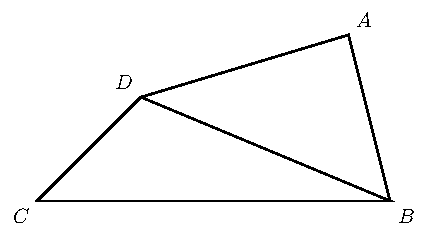
\includegraphics[height=4cm,page=1]{2021-07-17-figure-01}
\end{center}

\nopagebreak

\fbox{(A) $11$ \quad (B) $12$ \quad (C) $13$ \quad (D) $14$ \quad (E) $15$}

\begin{answer}
By the triangle inequality, 
\begin{align*}
     BD & < DA + AB \\
BD + DC & > BC
\end{align*}
And therefore
\begin{align*}
    BC - DC & < BD < DA + AB \\
12 = 17 - 5 & < BD < 9 + 5 = 14
\end{align*}
The answer is therefore
\begin{empheq}[box={\mathbox[colback=white]}]{equation*}
    13
\end{empheq}
\end{answer}
%%%%%%%%%%%%%%%%%%%%%%%%%%%%%%%%%%%%%%%%%%%%%%%%%%%%%%%%%%%%%%%%%%%%%%%%

\iftoggle{showAnswers}{\newpage}

%%%%%%%%%%%%%%%%%%%%%%%%%%%%%%%%%%%%%%%%%%%%%%%%%%%%%%%%%%%%%%%%%%%%%%%%
\subsection*{2.}

\nopagebreak

Rectangle $ABCD$ has $AB = 4$ and $BC = 3$. Segment $EF$ is constructed through $B$ so that $EF \perp DB$, and $A$ and $C$ lie on $DE$ and $DF$, respectively. What is $EF$?

\nopagebreak

\fbox{(A) $9$ \quad (B) $10$ \quad (C) $\dfrac{125}{12}$ \quad (D) $\dfrac{103}{9}$ \quad (E) $12$}

\begin{answer}
\begin{center}
  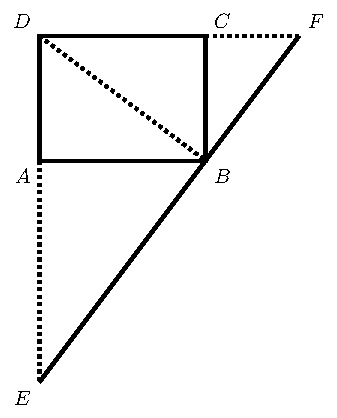
\includegraphics[height=7cm,page=1]{2021-07-17-figure-02}
\end{center}
\subsubsection*{Solution 1}
Let $D$ be the origin $(0,0)$ of a Cartesian system. The other points have the following coordinates: $A:(0,-3)$, $B:(4,-3)$, $C:(3,0)$. Line $DB$ has a zero-intercept and equation
\begin{align*}
y = -\frac{3x}{4}
\end{align*}
Since $EF$ is orthogonal to $DB$, it has slope $4/3$ (``minus the inverse''). And, since it goes through point $B(4,-3)$, $EF$ has intercept $-3-16/3$, and equation:
\begin{align*}
y = -\frac{25}{3} + \frac{4x}{3}
\end{align*}
Point $E$ is on the $y$ axis, with coordinates $\left(0,-\dfrac{25}{3}\right)$. 
Point $F$ is on the $x$ axis, with coordinates $\left(\dfrac{25}{4},0\right)$. 
The length of segment $EF$ is then
\begin{align*}
\left(\frac{25}{4}\right)^2 + \left(\frac{25}{3}\right)^2
  = \frac{125}{12}
\end{align*}
\end{answer}

\newpage
\begin{answer}
\subsubsection*{Solution 2}
The \textit{right-triangle altitude theorem} also known as the \textit{geometric mean theorem} states that the altitude $h$ is related to the $p$ and $q$ segments on the hypotenuse by
\begin{align*}
h = \sqrt{pq}
\end{align*}
In the figure, the area of the square, $h^2$, is equal to the area of the rectangle, $pq$.
\begin{center}
  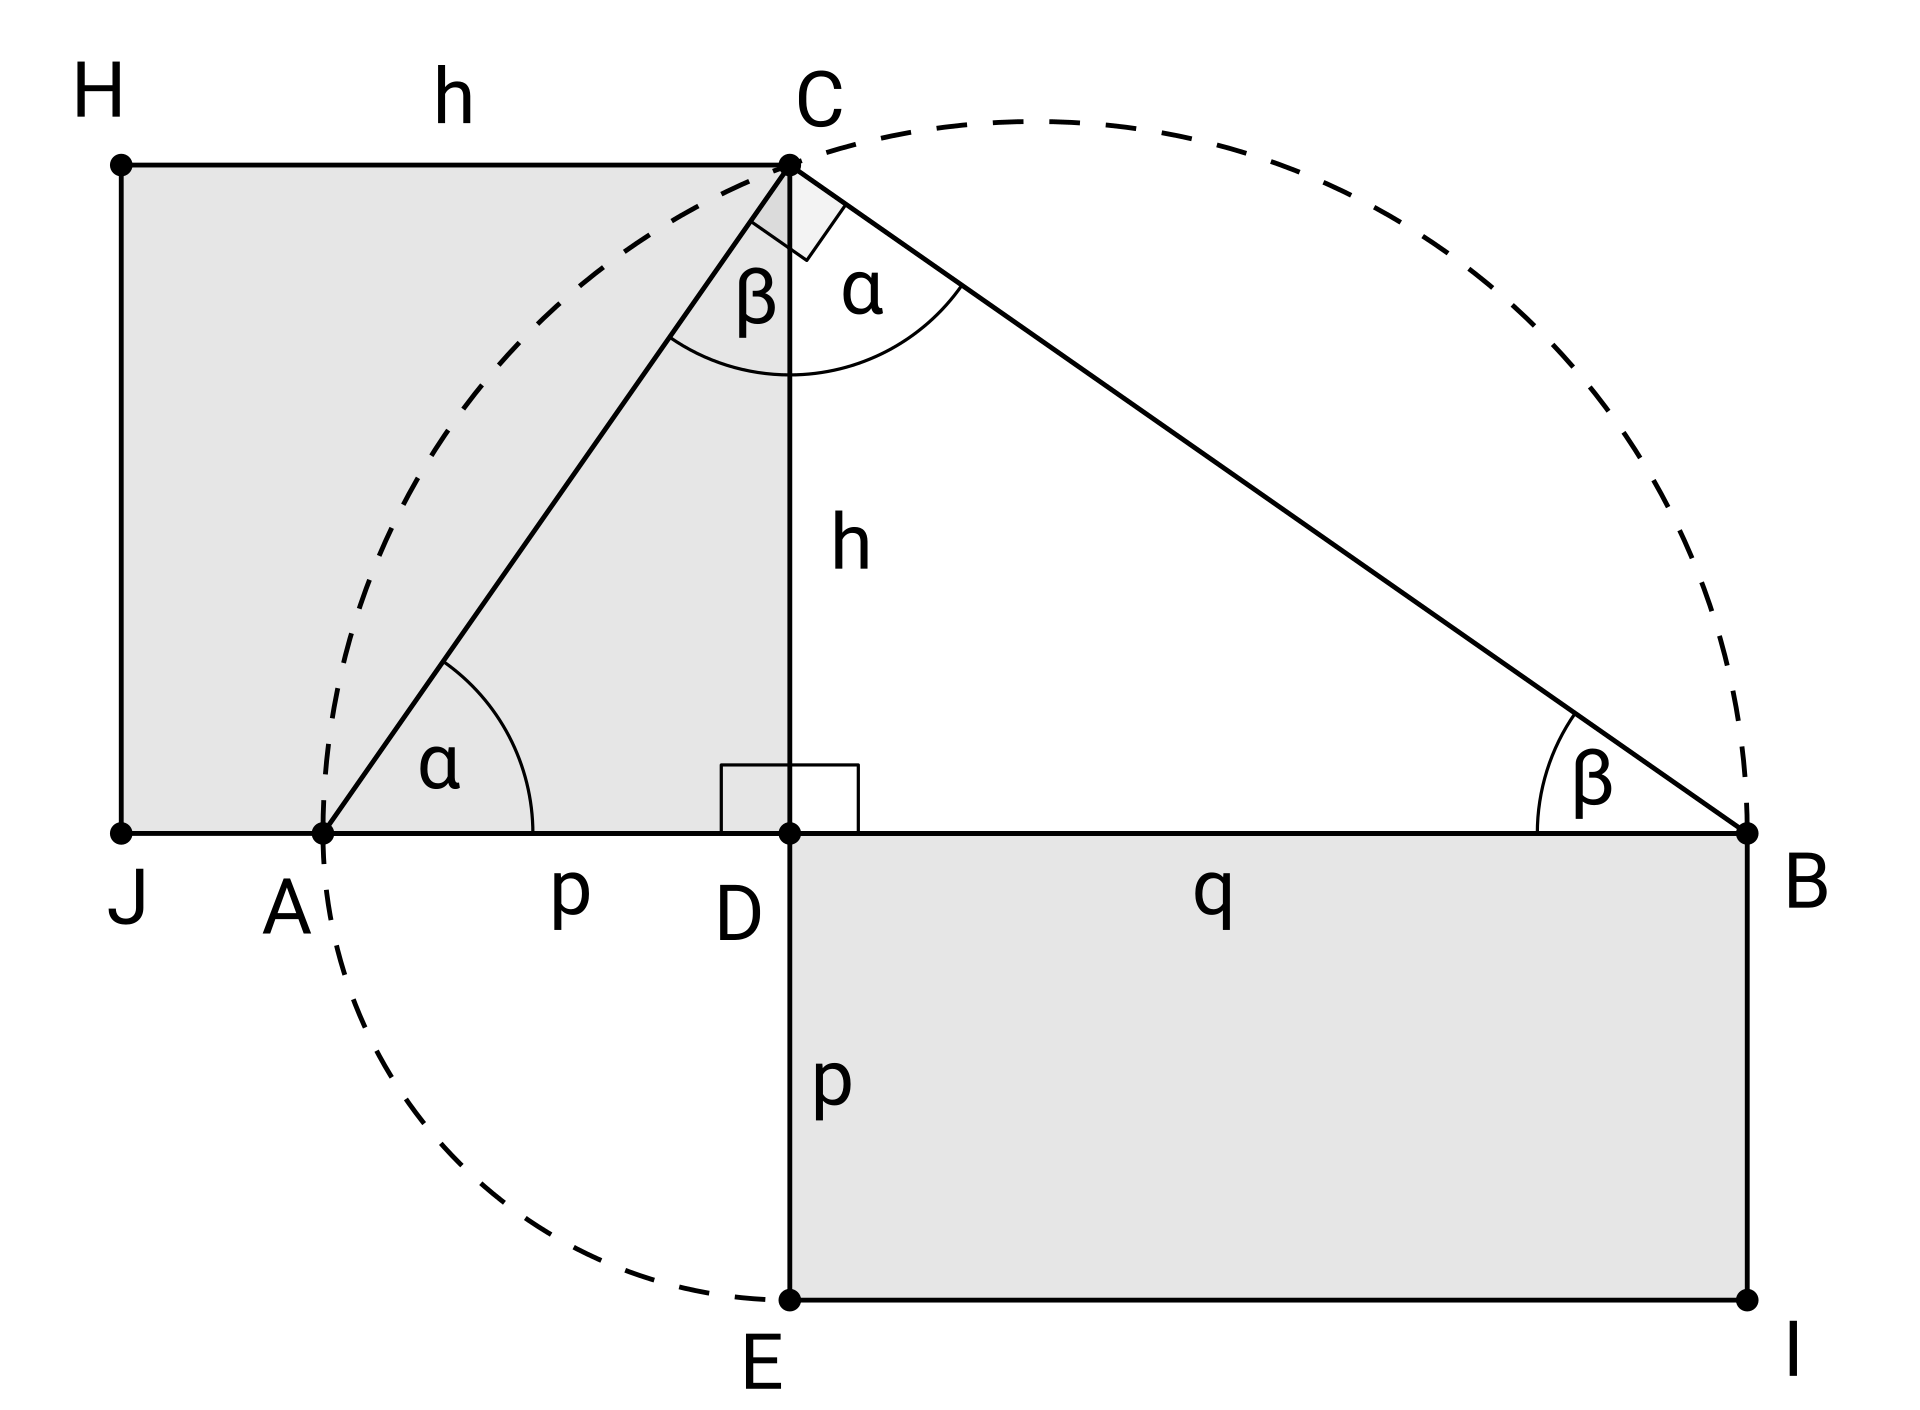
\includegraphics[height=7cm]{geometric-mean-theorem}
\end{center}
\bigskip
Here $h=DB$, $p=BF$, $q=BE$ and thus
\begin{align*}
DB^2 = BF \times BE
\end{align*}
Triangles $EBD$ and $DCB$ are similar, implying
\begin{align*}
\frac{BA}{BC} = \frac{BE}{BD} 
\implies
BE = \frac{BD \times BA}{BC}
   = \frac{5 \times 4}{3}
   = \frac{20}{3}
\end{align*}
where $BD=\sqrt{3^2+4^2}=5$ follows from the well-known Pythagorean triple. Now $BF$ follows from the geometric mean theorem, 
\begin{align*}
BF = \frac{DB^2}{BE} 
   = 5^2 \times \frac{3}{20}
   = \frac{15}{4}
\end{align*}
And lastly,
\begin{align*}
EF = BE + BF 
   = \frac{20}{3} + \frac{15}{4} 
   = \frac{80 + 45}{12} 
   = \frac{125}{12}
\end{align*}
\begin{empheq}[box={\mathbox[colback=white]}]{equation*}
    \frac{125}{12}
\end{empheq} 
\end{answer}
%%%%%%%%%%%%%%%%%%%%%%%%%%%%%%%%%%%%%%%%%%%%%%%%%%%%%%%%%%%%%%%%%%%%%%%%

\iftoggle{showAnswers}{\newpage}

%%%%%%%%%%%%%%%%%%%%%%%%%%%%%%%%%%%%%%%%%%%%%%%%%%%%%%%%%%%%%%%%%%%%%%%%
\subsection*{3.}

\nopagebreak

Points $A$, $B$, $C$, $D$, $E$, and $F$ lie, in that order, on $AF$, dividing it into five segments, each of length 1. Point $G$ is not on line $AF$. Point $H$ lies on $GD$, and point $J$ lies on $GF$. The line segments $HC$, $JE$, and $AG$ are parallel. Find $HC/JE$.

\nopagebreak

\begin{center}
  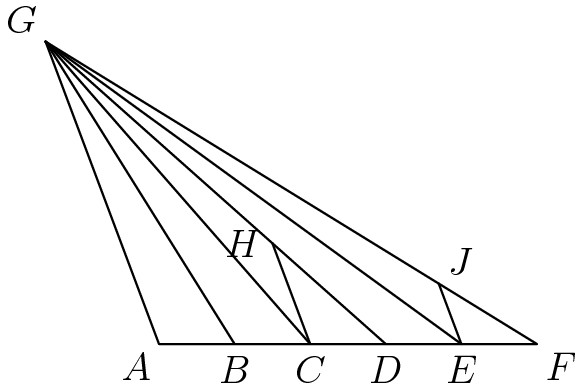
\includegraphics[height=5cm,page=1]{2021-07-17-figure-03}
\end{center}

\nopagebreak

\fbox{(A) $5/4$ \quad (B) $4/3$ \quad (C) $3/2$ \quad (D) $5/3$ \quad (E) $2$}

\begin{answer}
Since $AG$ and $CH$ are parallel, triangles $\triangle GAD$ and $\triangle HCD$ are similar, implying
\begin{align*}
\frac{CH}{AG} 
  = \frac{CD}{AD} 
  = \frac{1}{3}
\end{align*}

Since $AG$ and $JE$ are parallel, triangles $\triangle GAF$ and $\triangle JEF$ are similar, implying 
\begin{align*}
\frac{EJ}{AG} 
  = \frac{EF}{AF} 
  = \frac{1}{5}
\end{align*}
Putting it together,
\begin{align*}
\frac{CH}{EJ} 
  = \frac{CH}{AG} \times \frac{AG}{EJ}
  = \frac{5}{3}
\end{align*}
\begin{empheq}[box={\mathbox[colback=white]}]{equation*}
    \frac{5}{3}
\end{empheq} 
\end{answer}
%%%%%%%%%%%%%%%%%%%%%%%%%%%%%%%%%%%%%%%%%%%%%%%%%%%%%%%%%%%%%%%%%%%%%%%%

\iftoggle{showAnswers}{\newpage}

%%%%%%%%%%%%%%%%%%%%%%%%%%%%%%%%%%%%%%%%%%%%%%%%%%%%%%%%%%%%%%%%%%%%%%%%
\subsection*{4.}

\nopagebreak

In rectangle $ABCD$, $AB = 5$ and $BC = 3$. Points $F$ and $G$ are on $CD$ so that $DF = 1$ and $GC = 2$. Lines $AF$ and $BG$ intersect at $E$. Find the area of triangle $AEB$.

\nopagebreak

\begin{center}
  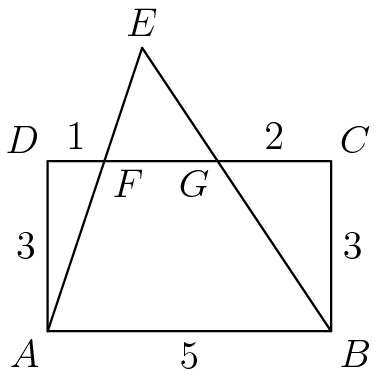
\includegraphics[height=5cm,page=1]{2021-07-17-figure-04}
\end{center}

\nopagebreak

\fbox{(A) $10$ \quad (B) $\dfrac{21}{2}$ \quad (C) $12$ \quad (D) $\dfrac{25}{2}$ \quad (E) $15$}

\begin{answer}
\subsubsection*{Solution 1}
Since $FG$ and $AB$ are parallel, triangles $\triangle EFG$ and $\triangle EAB$ are similar, implying 
\begin{align*}
\frac{\triangle EFG}{\triangle EAB}
  = \frac{FG}{AB}
  = \frac{2}{5}
\end{align*}
Let $h$ denote the height of $\triangle AEB$. Since $h$ is perpendicular to $FG$ and $AB$, we have
\begin{align*}
\frac{h-3}{h} = \frac{2}{5}
\implies
2h = 5h-15 
\implies
 h = 5
\end{align*}
The height is $5$ so the area of $\triangle EAB$ is 
\begin{align*}
\frac{1}{2} \times 5 \times 5 
  = \frac{25}{2}
\end{align*}
\end{answer}

\begin{answer}
\subsubsection*{Solution 2}
Let $A$ be the origin $(0,0)$ of a Cartesian system. 
Segments $EA$ and $EB$ have equation
\begin{align*}
y & = 3x \\
y & = \frac{15}{2} - \frac{3}{2}\, x 
\end{align*}
The $x$ coordinate of point $E$ solves the system:
\begin{align*}
y = 3x = \frac{15}{2} - \frac{3}{2}\, x
\implies
     x = \frac{5}{3},
\quad
     y = 5
\end{align*}
Thus, the area of $\triangle EAB$ is 
\begin{empheq}[box={\mathbox[colback=white]}]{equation*}
    \frac{25}{2}
\end{empheq} 
\end{answer}
%%%%%%%%%%%%%%%%%%%%%%%%%%%%%%%%%%%%%%%%%%%%%%%%%%%%%%%%%%%%%%%%%%%%%%%%

\iftoggle{showAnswers}{\newpage}

%%%%%%%%%%%%%%%%%%%%%%%%%%%%%%%%%%%%%%%%%%%%%%%%%%%%%%%%%%%%%%%%%%%%%%%%
\subsection*{5.}

\nopagebreak

Points $E$ and $F$ are located on square $ABCD$ so that triangle $BEF$ is equilateral. What is the ratio of the area of triangle $DEF$ to that of triangle $ABE$?

\nopagebreak

\begin{center}
  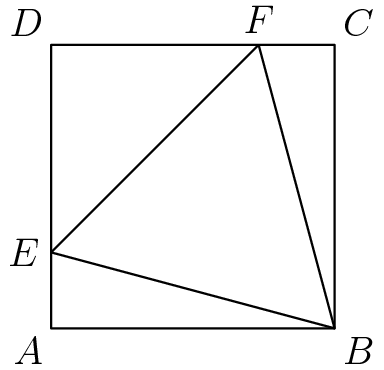
\includegraphics[height=5cm,page=1]{2021-07-17-figure-05}
\end{center}

\nopagebreak

\fbox{(A) $\dfrac{4}{3}$ \quad (B) $\dfrac{3}{2}$ \quad (C) $\sqrt{3}$ \quad (D) $2$ \quad (E) $1+\sqrt{3}$}

\begin{answer}
Without loss of generality, suppose the side length of square $ABCD$ is $1$. 
Triangles $\triangle ABE$ and $\triangle CBF$ are congruent and since $BE=BF$, it follows that $CF=AE$ and $DE=DF$. Let $DE=x$. $EF$ is the diagonal of a square of side length $x$, so that
\begin{align*}
EF = x \sqrt{2}
\end{align*}
Consider now $\triangle ABE$. Its side lengths are $AB=1$, $BE=EF=x\sqrt{2}$, $AE=1-x$. By the Pythagorean Theorem, 
\begin{align*}
AE^2 + AB^2 & = BE^2 \\
(1-x)^2 + 1 & = 2x^2
\end{align*}
This gives $x^2 = 2(1-x)$ and the implied ratio
\begin{align*}
\frac{[DEF]}{[ABE]}
  = \frac{\dfrac{x^2}{2}}{\dfrac{1-x}{2}} 
  = \frac{x^2}{1-x} = 2
\end{align*}
\begin{empheq}[box={\mathbox[colback=white]}]{equation*}
  \frac{[DEF]}{[ABE]} = 2
\end{empheq} 

\end{answer}
%%%%%%%%%%%%%%%%%%%%%%%%%%%%%%%%%%%%%%%%%%%%%%%%%%%%%%%%%%%%%%%%%%%%%%%%

\iftoggle{showAnswers}{\newpage}

%%%%%%%%%%%%%%%%%%%%%%%%%%%%%%%%%%%%%%%%%%%%%%%%%%%%%%%%%%%%%%%%%%%%%%%%
\subsection*{6.}

\nopagebreak

In triangle $ABC$ points $D$ and $E$ lie on $BC$ and $AC$, respectively. If $AD$ and $BE$ intersect at $T$ so that $AT/DT = 3$ and $BT/ET = 4$, what is $CD/BD$?

\nopagebreak

\begin{center}
  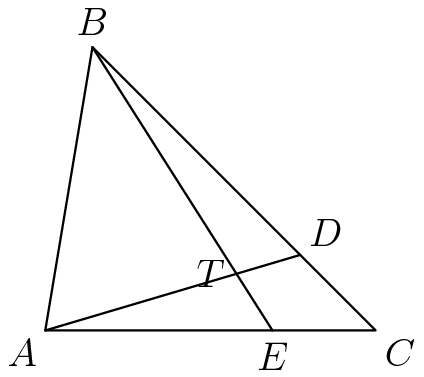
\includegraphics[height=5cm,page=1]{2021-07-17-figure-06}
\end{center}

\nopagebreak

\fbox{(A) $\dfrac{1}{8}$ \quad (B) $\dfrac{2}{9}$ \quad (C) $\dfrac{3}{10}$ \quad (D) $\dfrac{4}{11}$ \quad (E) $\dfrac{5}{12}$}

\begin{answer}
Since triangles $\triangle ADC$ and $\triangle ADB$ have segment $AD$ in common, the ratio of segments $CD$ and $BD$ is equal to the ratio of the areas:
\begin{align*}
\frac{CD}{BD}
 = \frac{[\triangle ADC]}{[\triangle ADB]}
\end{align*}
These triangles are made up of several pieces. First, express $\triangle ADB$  in terms of $[\triangle BTD]$.
\begin{align*}
[\triangle ATB] = 3 \, [\triangle BTD]
\end{align*}
Since we are interested in ratios, we let $[\triangle BTD] = 1$ without loss of generality. 
\begin{align*}
[\triangle ADB] = [\triangle ATB] + [\triangle BTD] = 4 \, [\triangle BTD] = 4
\end{align*}
Secondly, express $[\triangle ADC]$ in terms of $[\triangle BTD]$.
\begin{align*}
[\triangle ADC] 
  & = [\triangle ATE] + [\triangle TDCE] \\
  & = [\triangle ATE] + [\triangle TCD] + [\triangle TCE] \\
  & = [\triangle ATE] + [\triangle TCD] + [\triangle TCE]
\end{align*}
$[\triangle ATE]$ is readily calculated, with more work needed for $[\triangle TCD]$ and $[\triangle TCE]$.
\begin{align*}
[\triangle ATE] & = \frac{3}{4} \, [\triangle BTD] = \frac{3}{4}
\end{align*}
Let $x = [\triangle TCD]/[\triangle BTD]$ and $y = [\triangle TCE]/[\triangle BTD]$. 
\begin{align*}
\frac{[\triangle BTC]}{[\triangle TCE]} 
 & = \frac{1+x}{y}  = 4 
\implies 
 x - 4y = -1 \\
\frac{[\triangle ATC]}{[\triangle TCD]} 
 & = \frac{\dfrac{3}{4}+y}{x} = 3
\implies 
 12x - 4y = 3
\end{align*}
Solving the system for $x$ and $y$ yields
\begin{align*}
[\triangle TCD] / [\triangle BTD] & = \frac{4}{11} \\[1ex]
[\triangle TCE] / [\triangle BTD] & = \frac{15}{44}
\end{align*}
Putting it together:
\begin{align*}
[\triangle ADC] / [\triangle BTD] 
  & = \frac{3}{4} + \frac{4}{11} + \frac{15}{44}
    = \frac{33+16+15}{44}
    = \frac{64}{44}
\end{align*}
and thus,
\begin{align*}
\frac{CD}{BD} 
  = \dfrac{64}{44} \div 4
  = \frac{4}{11}
\end{align*}

\begin{empheq}[box={\mathbox[colback=white]}]{equation*}
    \frac{4}{11}
\end{empheq} 
\end{answer}
%%%%%%%%%%%%%%%%%%%%%%%%%%%%%%%%%%%%%%%%%%%%%%%%%%%%%%%%%%%%%%%%%%%%%%%%

\iftoggle{showAnswers}{\newpage}

%%%%%%%%%%%%%%%%%%%%%%%%%%%%%%%%%%%%%%%%%%%%%%%%%%%%%%%%%%%%%%%%%%%%%%%%
\subsection*{7.}

\nopagebreak

Triangle $ABC$ has a right angle at $B$, $AB = 1$, and $BC = 2$. The bisector of $\angle BAC$ meets $BC$ at $D$. What is $BD$?

\nopagebreak

\begin{center}
  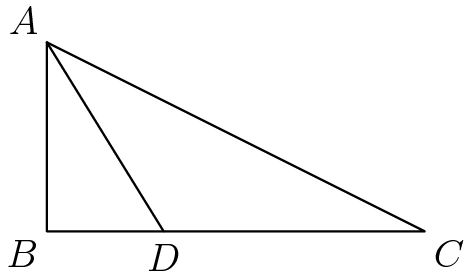
\includegraphics[height=3cm,page=1]{2021-07-17-figure-07}
\end{center}

\nopagebreak

\fbox{(A) $\dfrac{\sqrt{3}-1}{2}$ \quad (B) $\dfrac{\sqrt{5}-1}{2}$ \quad (C) $\dfrac{\sqrt{5}+1}{2}$ \quad (D) $\dfrac{\sqrt{6}+\sqrt{2}}{2}$ \quad (E) $2\sqrt{3}-1$}

\begin{answer}
By the Pythagorean Theorem, 
\begin{align*}
AC = \sqrt{5}
\end{align*}
By the Angle Bisector Theorem,
\begin{align*}
\frac{BD}{AB} 
  = \frac{DC}{AC}
\end{align*}
Substituting the known lengths,
\begin{align*}
\frac{BD}{1} 
  & = \frac{2-BD}{\sqrt{5}} \\[1ex]
\left(1+\frac{1}{\sqrt{5}}\right) \, BD
  & = \frac{2}{\sqrt{5}} \\[1ex]
BD & = \frac{2}{\sqrt{5}+1}
 = \frac{2(\sqrt{5}-1)}{(\sqrt{5}+1)(\sqrt{5}-1)}
 = \frac{\sqrt{5}-1}{2}
\end{align*}
\begin{empheq}[box={\mathbox[colback=white]}]{equation*}
    \frac{\sqrt{5}-1}{2}
\end{empheq} 
\end{answer}
%%%%%%%%%%%%%%%%%%%%%%%%%%%%%%%%%%%%%%%%%%%%%%%%%%%%%%%%%%%%%%%%%%%%%%%%

\iftoggle{showAnswers}{\newpage}

%%%%%%%%%%%%%%%%%%%%%%%%%%%%%%%%%%%%%%%%%%%%%%%%%%%%%%%%%%%%%%%%%%%%%%%%
\subsection*{8.}

\nopagebreak

Right triangle $ABC$ has $AB = 3$, $BC = 4$, and $AC = 5$. Square $XYZW$ is inscribed in triangle $ABC$ with $X$ and $Y$ on $AC$, $W$ on $AB$, and $Z$ on $BC$. What is the side length of the square?

\nopagebreak

\begin{center}
  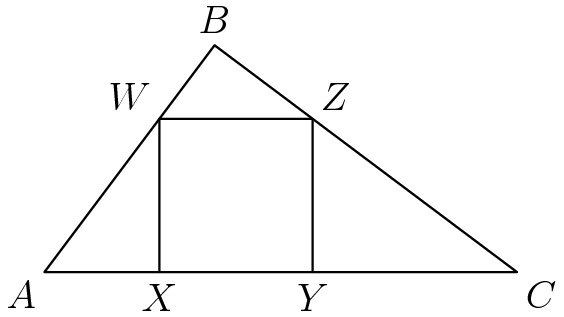
\includegraphics[height=3cm,page=1]{2021-07-17-figure-08}
\end{center}

\nopagebreak

\fbox{(A) $\dfrac{3}{2}$ \quad (B) $\dfrac{60}{37}$ \quad (C) $\dfrac{12}{7}$ \quad (D) $\dfrac{23}{13}$ \quad (E) $2$}

\begin{answer}
Let $a$ be the side length of the inscribed square. 

Triangles $\triangle ACB$ and $\triangle WZB$ are congruent, implying
\begin{align*}
\frac{ZB}{ZW} 
  = \frac{CB}{CA} 
  = \frac{4}{5} 
\implies
  ZB = \frac{4a}{5}
\end{align*}
Triangles $\triangle CBA$ and $\triangle ZYC$ are congruent, implying
\begin{align*}
\frac{ZC}{ZY}
  = \frac{AC}{AB} 
  = \frac{5}{3}
\implies
  ZC = \frac{5a}{3}
\end{align*}
It follows that
\begin{align*}
CB & = ZB + ZC \\[1ex]
4  & = \dfrac{4a}{5} + \dfrac{5a}{3} 
     = \dfrac{37a}{15} \\[1ex]
 a & = 4 \times \frac{15}{37}
     = \frac{60}{37} 
\end{align*}
\begin{empheq}[box={\mathbox[colback=white]}]{equation*}
    \frac{60}{37}
\end{empheq} 
\end{answer}
%%%%%%%%%%%%%%%%%%%%%%%%%%%%%%%%%%%%%%%%%%%%%%%%%%%%%%%%%%%%%%%%%%%%%%%%

\iftoggle{showAnswers}{\newpage}

%%%%%%%%%%%%%%%%%%%%%%%%%%%%%%%%%%%%%%%%%%%%%%%%%%%%%%%%%%%%%%%%%%%%%%%%
\subsection*{9.}

\nopagebreak

A triangle with sides of $5$, $12$, and $13$ has both an inscribed and a circumscribed circle. What is the distance between the centers of those circles?

\nopagebreak

\fbox{(A) $\dfrac{3\sqrt{5}}{2}$ \quad (B) $\dfrac{7}{2}$ \quad (C) $\sqrt{15}$ \quad (D) $\dfrac{\sqrt{65}}{2}$ \quad (E) $\dfrac{9}{2}$}

\begin{answer}
Pick a coordinate system so that the right angle is at
Let $A$ be the center $(0,0)$ of a coordinate system such that the vertices $B$ and $C$ have coordinates $(12,0)$ and $(0,5)$.
This is a right triangle --- it is a well-known Pythagorean triple. This means that the center of the circumscribed circle is on the hypotenuse at the middle point, at coordinates $(6,2.5)$. 
\bigskip
\begin{center}
  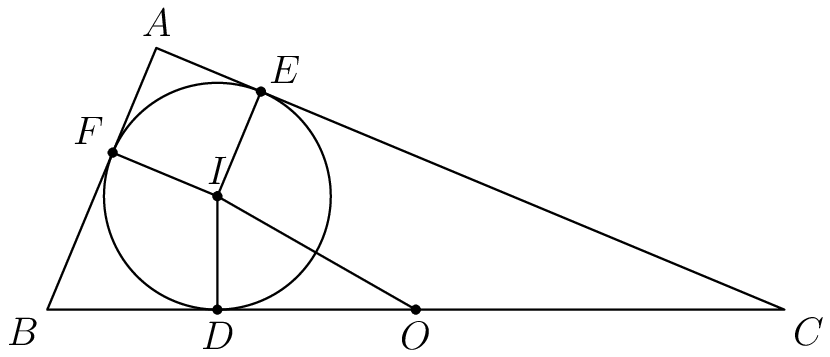
\includegraphics[height=8cm,page=1]{2021-07-17-figure-09}
\end{center}
\bigskip
Let $A$ be the area of the triangle, let $P$ be its perimeter, and let $r$ be the radius of the inscribed circle. These quantities are related by the identity
\begin{align*}
r = \frac{A}{\sfrac{1}{2}\,P}
\end{align*}
For this particular triangle, we have
\begin{align*}
P & = 5 + 12 + 13 = 30 \\[1ex]
A & = \frac{5 \times 12}{2} = 30
\end{align*}
implying $r=2$. The coordinates of the center are therefore $(r,r)=(2,2)$. 

The distance between the center of the circumscribed circle $(6,2.5)$ and the center of the inscribed circle $(2,2)$ is
\begin{align*}
\sqrt{(6-2)^2 + (2.5-2)^2}
  = \sqrt{16.25} 
  = \frac{\sqrt{65}}{2}
\end{align*}
\begin{empheq}[box={\mathbox[colback=white]}]{equation*}
    \frac{\sqrt{65}}{2}
\end{empheq} 
\end{answer}
%%%%%%%%%%%%%%%%%%%%%%%%%%%%%%%%%%%%%%%%%%%%%%%%%%%%%%%%%%%%%%%%%%%%%%%%

\iftoggle{showAnswers}{\newpage}

%%%%%%%%%%%%%%%%%%%%%%%%%%%%%%%%%%%%%%%%%%%%%%%%%%%%%%%%%%%%%%%%%%%%%%%%
\subsection*{10.}

\nopagebreak

In triangle $ABC$ we have $AB = 25$, $BC = 39$, and $AC = 42$. Points $D$ and $E$ are on $AB$ and $AC$ respectively, with $AD = 19$ and $AE = 14$. What is the ratio of the area of triangle $ADE$ to the area of the quadrilateral $BCED$?

\nopagebreak

\fbox{(A) $\dfrac{266}{1521}$ \quad (B) $\dfrac{19}{75}$ \quad (C) $\dfrac{1}{3}$ \quad (D) $\dfrac{19}{56}$ \quad (E) $1$}

\begin{answer}
Consider
\bigskip
\begin{center}
  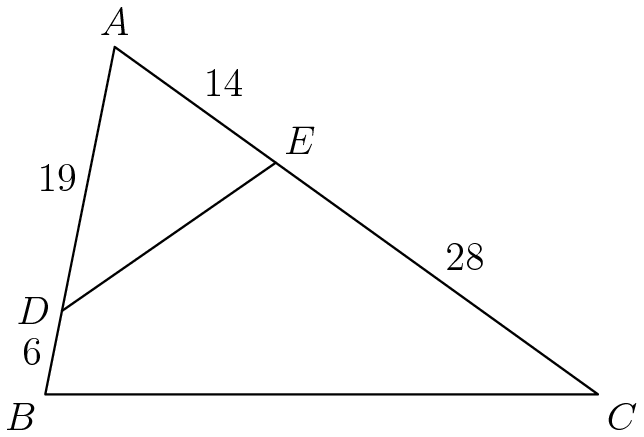
\includegraphics[height=5cm,page=1]{2021-07-17-figure-10}
\end{center}
\bigskip
We have that 
\begin{align*}
\frac{[ADE]}{[ABC]} 
  = \frac{AD}{AB} \cdot \frac{AE}{AC} 
  = \frac{19}{25} \cdot \frac{14}{42} 
  = \frac{19}{75}.
\end{align*}
But $[BCED] = [ABC] - [ADE]$, so 
\begin{align*} 
\frac{[ADE]}{[BCED]} 
 & = \frac{[ADE]}{[ABC] - [ADE]} \\ 
 & = \frac{1}{[ABC]/[ADE] - 1} \\ 
 & = \frac{1}{75/19 - 1} \\ 
 & = \frac{19}{56}
\end{align*}
\begin{empheq}[box={\mathbox[colback=white]}]{equation*}
    \frac{19}{56}
\end{empheq} 
\end{answer}
%%%%%%%%%%%%%%%%%%%%%%%%%%%%%%%%%%%%%%%%%%%%%%%%%%%%%%%%%%%%%%%%%%%%%%%%

\end{document}
